\section{Введение}

Ядерная физика обогатила науку новыми знаниями и позволила глубже проникнуть в тайны природы. Идеи и факты, полученные при изучении ядерных процессов, меняют наши представления об окружающем мире. Концепции, развитые в ядерной физике, позволили понять образование химических элементов и их изотопов, процессы энергетики Солнца, параметры нейтронных звезд и многое другое. Ядерная физика нашла широкое применение в энергетике, в различных областях науки, ускорила научно-технический прогресс. Поэтому, развитие этой науки является одной из важнейших задач человечества.

\subsection{Экзотические ядра}

Атомные ядра представляют собой связанные квантовые системы фермионов. Свойства атомных ядер определяются совместным действием сильного, электромагнитного и слабого взаимодействий. Известно, что существует 254 стабильных изотопа, однако природе мы можем обнаружить 339 изотопов\cite{ufn}, то есть, некоторые нестабильные изотопы живут достаточно долго, чтобы дожить до нас с времён образования вселенной, или как продукты распада ядер-предшественников. C точки зрения ядерной физики, понятие "стабильность" означает устойчивость относительно сильного взаимодействия. В настоящее время обнаружено примерно 3100 различных изотопов\cite{ufn}, представляющих собой различные сочетания чисел протонов Z и нейтронов N. Говорить о точном количестве изотопов не имеет смысла, так как исследования в поиске новых изотопов не прекращаются по сей день, поэтому ежегодно число известных изотопов увеличивается на 3-10 единиц. Теоретические предсказания таковы, что, вероятно, могут существовать ещё около 2000-3000 пока неизвестных стабильных изотопов\cite{ufn}. 

На Рис.~\ref{ris:NuclearMap} показана N-Z диаграмма атомных ядер. Чёрными точками обозначены самые стабильные ядра. (Для таких ядер  значение N/Z имеет значение, определяемое равновесием ядерных и кулоновских сил в ядре) Область расположения стабильных ядер обычно называют долиной стабильности. Для ядер долины стабильности характерно отношение числа нейтронов к числу протонов.

$$N/Z = 0.98 + 0.015 \cdot A^{2/3},$$
где $N$ - количество нейтронов, $Z$ - количество протонов в ядре. $A = Z + N$ - массовое число\cite{inet}.

{
	\centering
	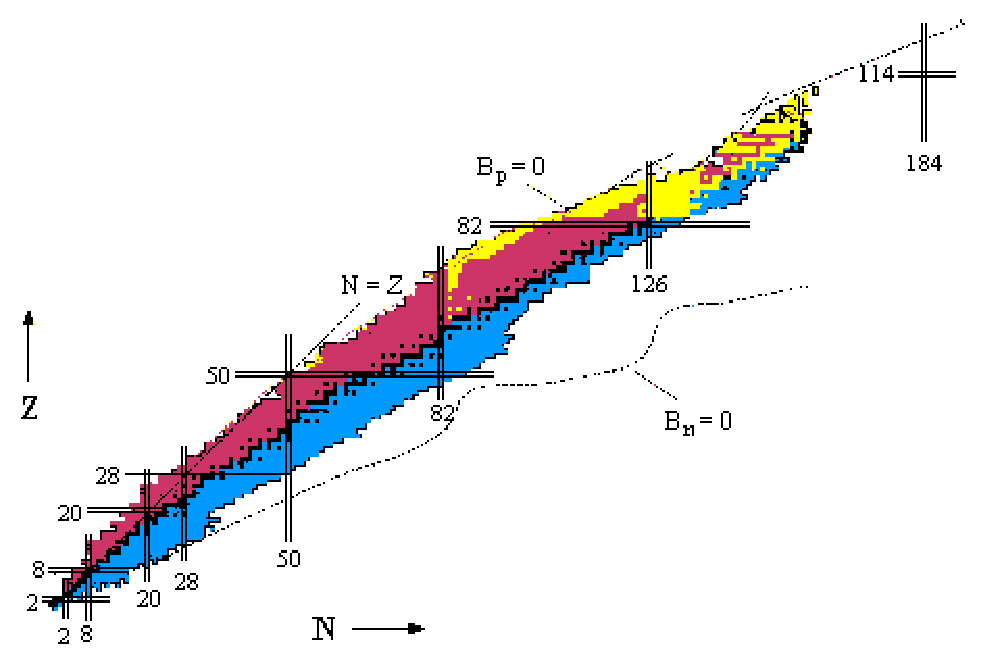
\includegraphics[width=1\linewidth]{NuclearMap.eps}
	\captionof{figure}{Карта ядерной стабильности\cite{inet}}\label{ris:NuclearMap}
}

%\begin{figure}[h]
%	\center{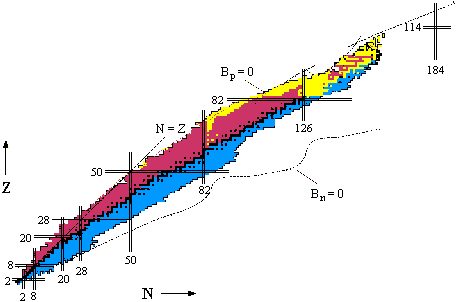
\includegraphics[width=1\linewidth]{NuclearMap.png}}
%	\caption{Карта ядерной стабильностиp\cite{inet}}
%	\label{ris:NuclearMap}
%\end{figure}

По особенностям свойств ядра делят на легкие (А<12-16), средние (А<200) и тяжелые (выше А>200). Легкие стабильные ядра имеют приблизительно равные числа нейтронов и протонов. В области более тяжелых ядер отношение числа нейтронов к числу протонов начинает возрастать и достигает величины 1.6 в районе А=250. Это изменение можно объяснить учитывая короткодействующий характер ядерных сил и возрастающую роль кулоновского взаимодействия протонов с ростом зарядового числа Z. Тяжелые ядра оказываются энергетически более устойчивыми, если содержат большее число нейтронов N по сравнению с числом протонов Z. Известно, что для стабильных ядер средняя энергия связи на нуклон принимает значение $\bar{E}\sim8$ МэВ на нуклон \cite{inet}. По мере отдаления от долины стабильности, энергия связи выбранного ядра уменьшается, тем самым, испускание нуклона выбранным ядром становится более вероятным, при его возбуждении. Пунктирные линии (см. Рис.1) очерчивают область возможного существования атомных ядер. Связанное состояние ядра определяется как состояние, связанное относительно испускания нейтронов или протонов, т.е. считается, что атомное ядро существует, если оно не испускает нуклоны из основного состояния. Линия $B_p$ = 0 ($B_p$ - энергия отделения протона) ограничивает область стабильных ядер слева (proton drip-line). Линия $B_n$ = 0 ($B_n$ - энергия отделения нейтрона) - справа (neutron drip-line). Ядра, сильно пререгруженные нейтронами или протонами, лежащие близко к границе стабильности, называются экзотическими ядрами.

В случае экзотических ядер могут наблюдаться такие явления, как нейтронное гало, мягкая мода дипольного возбуждения и другие. 

Явление нейтронного гало заключается в следующем: малая величина энергии связи  валентного нейтрона (или группы нейтронов) и короткодействующий характер ядерных сил  приводят к туннелированию нейтронов во внешнюю область ядра на большие расстояния от его кора. В таком случае, плотность распределения нейтронов на периферии намного меньше плотности распределения нейтронов кора. Нейтроны периферии могут быть удалены от кора на очень большие расстояния, что приводит к увеличению среднеквадратичного радиуса относительно радиуса стабильных ядер с таким же количеством нуклонов. Например, среднеквадратичный радиус распределения валентных нуклонов в $^{11}$Li сравним с радиусом ядра $^{208}$Pb.

В случае ядер $^8$He, $^6$Be имеет место такое явление, как мягкая мода дипольного возбуждения, которое связано с колебаниями валентных нуклонов относительно кора.

Также изменение соотношения числа нейтронов к числу протонов (N/Z) может привести к изменению оболочечной структуры ядра – вместо известных магических чисел (2, 8, 20...) могут появляться новые.

\subsection{Образование экзотических ядер}


В лабораторных условиях получать ядра вблизи границы стабильности сложно из-за малых сечений образования этих ядер и коротких периодов полураспада. В настоящее время методы сепарации и детектирования образующихся в результате ядерных реакций экзотических ядер достигли такого уровня, что основные характеристики атомных ядер: масса, период полураспада, основные моды распада - могут быть получены на основе анализа небольшого числа ядер(например \cite{flnr}).

Одним из способов изучения экзотических ядер являются эксперименты с использованием радиоактивных пучков. Проблема получения таких пучков заключается в том, что эти ядра, как правило,  имеют короткие (менее 1 секунды) времена жизни, что делает невозможным использование традиционных методов, применяемых для получения пучков стабильных ядер. В связи с этим возникла необходимость разработки специальных методов выделения требуемого изотопа из спектра вторичных частиц, который образуется в результате взаимодействия первичного пучка с мишенью.

Существует два основных метода получения пучков радиоактивных ядер.
Исторически первым методом работы с пучками радиоактивных изотопов стал метод ISOL (Isotope Separation On-Line)\cite{ufn}. Ядро-мишень разрушается в реакции расщепления лёгкими налетающими частицами. Мишень сделана таким образом, что продукты реакции застревают в её объеме. Далее, нужные изотопы определенным способом извлекаются из мишени, проходят сепарацию и ионизацию. После сепарации пучок радиоактивных частиц имеет кинетическую энергию в диапазоне от 10 до 500 КэВ и может быть использован в экспериментах с низкими энергиями, или может быть направлен в ускоритель вторичных частиц, если время жизни ядер это позволяет. В последнем случае качество вторичного пучка определяется параметрами соответствующего ускорителя и не отличается от качества стандартных пучков стабильных ядер. Времена извлечения радиоактивных ядер из мишени и их транспортировка ко второму ускорителю определяют диапазон времен жизни экзотических ядер, для которых может быть использован этот метод. Современные ISOL-методы уверенно обеспечивают время выделения порядка 100мс\cite{ufn}. 
%Преимущество ISOL состоит в том, что этот метод не требует дополнительной диагностики свойств пучка.

Значительными преимуществами по времени выделения и интенсивности пучков радиоактивных изотопов обладает метод разделения на лету (In-Flight Separation). В этом методе пучок частиц с энергией от 30 МэВ/нуклон до 1 ГэВ/нуклон налетает на производящую мишень (в основном бериллиевую). В результате столкновения получается большое количество осколков-фрагментов, которые летят преимущественно по направлению первичного пучка и попадают во фрагмент-сепаратор, выделяющий частицы с определенным значением магнитной жесткости($\xi$), которая определяется отношением :

\begin{equation}
\label{Mag}
\xi = B \rho =  \frac{pc}{Ze},
\end{equation}

где $p$ - импульс частицы, $Z$ — атомный номер, $c$ – скорость света, $e$ – элементарный электрический заряд, $\rho$ - радиус кривизны траектории движения частицы, $B$ - вектор магнитной индукции.  На выходе фрагмент-сепаратора, в зависимости от степени очистки, помимо интересующего нас изотопа, мы имеем коктейль из примесных изотопов, имеющих близкие значения магнитной жесткости. Энергетическая дисперсия пучка определяется аксептансом фрагмент-сепаратора и составляет, как правило, величину порядка нескольких процентов от полной энергии пучка. 


%Существует два основных метода получения пучков радиоактивных ядер: 
%
%1. ISOL (Isotope Separation On Line). В этом методе, в отличие от In-Flight, процессы производства и ускорения экзотических ядер отделены друг от друга. Мишень сделана таким образом, что продукты реакции застревают в её объеме. Далее, нужные изотопы определенным способом извлекаются из мишени, проходят сепарацию и ионизацию. На выходе из сепаратора пучок радиоактивных частиц имеет энергию в диапазоне от 10 до 500 кэВ и может быть использован в экспериментах с низкими энергиями, или может быть направлен в ускоритель вторичных частиц. В последнем случае качество вторичного пучка определяется параметрами соответствующего ускорителя и не отличается от качества стандартных пучков стабильных ядер. Времена извлечения радиоактивных ядер из мишени и их транспортировка ко второму ускорителю определяют диапазон времен жизни экзотических ядер, для которых может быть использован этот метод. Преимущество ISOL состоит в том, что этот метод не требует дополнительной диагностики свойств пучка.
%
%2. In-Flight. Пучок частиц с энергией от 30 МэВ/нуклон до 1 ГэВ/нуклон налетает на производящую мишень (в основном бериллиевую). В результате столкновения получается большое количество осколков-фрагментов, которые летят преимущественно вперед и попадают во фрагмент-сепаратор, выделяющий частицы с определенным значением магнитной жесткости. На выходе фрагмент-сепаратора, в зависимости от степени очистки, помимо интересующего нас изотопа, мы имеем коктейль из примесных изотопов, имеющих близкие значения магнитной жесткости. Энергетическая дисперсия пучка определяется аксептансом фрагмент-сепаратора и составляет, как правило, величину порядка нескольких процентов от полной энергии пучка. 
%
Для пучков вторичных частиц, полученных более быстрым методом In-Flight, требуется диагностика свойств пучка, таких как энергия, состав и др.